\documentclass[conference]{IEEEtran}
\usepackage[spanish]{babel}
\usepackage[utf8]{inputenc}
\usepackage{blindtext, graphicx}
\usepackage{subfigure}
\usepackage{mdwmath}
\usepackage{mdwtab}
\usepackage{subfig}
\usepackage{amsmath}

\begin{document}
\title{ Detecci\'on de bordes utilizando filtros de primera derivada }
\author{\IEEEauthorblockN{Walter Alejandro Moreno Ram\'irez}
\IEEEauthorblockA{Departamento de Estudios Multidisciplinarios\\
Universidad de Guanajuato\\
Yuriria, Guanajuato\\
Correo: wa.morenoramirez@ugto.mx}}

\maketitle
\renewcommand\abstractname{Abstract}
\begin{abstract}
This article describes what are the edges of an image, as they can be detected by obtaining the gradient of a region of the image. Its advantages and applications will also be stated. \\\\
\end{abstract}

\begin{IEEEkeywords}
Pixel, convoluci\'on, filtros, gradiente, primera derivada, funci\'on, C++, OpenCV, ventana, m\'ascara, vecindario.
\end{IEEEkeywords}

\IEEEpeerreviewmaketitle
\section{Introducci\'on} 
Los bordes de una imagen digital se pueden definir como un cambio entre dos regiones de niveles de gris significativamente distintos, normalmente se toman las transiciones entre regiones con nivel de gris 0 a nivel de gris 255. Los bordes nos dan informaci\'on sobre las fronteras de los objetos y poder reconocerlos.\\\\
La derivada de una se\~nal continua proporciona las variaciones locales con respecto a una sola variable, de forma que el valor de la derivada es mayor cuanto m\'as r\'apidas son los cambios o transiciones de niveles de gris.\\
En el caso de funciones de dos variables $f(x,y)$, la derivada es un vector que apunta en la direcci\'on de la m\'axima variaci\'on de $f(x,y)$ y cuyo m\'odulo es proporcional a dicha variac\'on. Este vector se denomina gradiente y se define en la Ecuaci\'on (1).\\
\begin{equation}
	\nabla f(x,y) = \left[ f_{x}(x,y) \hat{i}, f_{y}(x,y)\hat{j} \right]
\end{equation}
\\
Cuya magnitud esta definida por la Ecuaci\'on (2).\\
\begin{equation}
	\parallel \nabla f(x,y) \parallel = \sqrt{ \left( f_{x}(x,y) \right) ^2 + \left( f_{y}(x,y) \right)^2 } 
\end{equation}
\\ Y su angulo esta dado por la Ecuaci\'on (3).\\
\begin{equation}
	\theta = \arctan\left(  \frac{f_{y}(x,y)}{f_{x}(x,y)} \right)
\end{equation}
\\

\section{Metodolog\'ia}
Un imagen digital se puede ver como una funci\'on de dos variables, pero al no existir un n\'umero infinito de p\'ixeles entre pares de p\'ixeles adyacentes ser\'a una funci\'on discreta. Para una funci\'on bidimensional discreta, las distintas aproximaciones del operador gradiente se basan en diferencias entre los niveles de grises de la imagen. La derivada parcial $f_{x}(x,y)$ (gradiente de fila $g_{f}(i,j)$) puede aproximarse por la diferencia de los p\'ixeles adyacentes de la misma fila. Se define por la ecuaci\'on (4).

\begin{equation}
	f_{x}(x,y) \approx \nabla_{x}f(x,y) = f(x,y)-f(x-1,y)
\end{equation}
\\ Lo que nos da como resultado un gradiente en forma de matriz fila como se muestra en la Figura 1.
\begin{figure}[h]
	\centering
	\setlength{\unitlength}{0.00105in}
	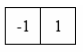
\includegraphics[scale=0.50]{./images/fx.png}	
	\caption{Matriz resultante de dicretizar en el eje x.}	
\end{figure}

La discretizaci\'on del vector gradiente en el eje Y ($G_{c}(i,j)$), se define en la Ecuaci\'on (5).\\
\begin{equation}
	f_{x}(x,y) \approx \nabla_{x}f(x,y) = f(x,y)-f(x-1,y)
\end{equation}
\\ Lo que nos da como resultado un gradiente en forma de matriz fila como se muestra en la Figura 1.
\begin{figure}[h]
	\centering
	\setlength{\unitlength}{0.00105in}
	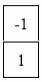
\includegraphics[scale=0.50]{./images/fy.png}	
	\caption{Matriz resultante de discretizar en el eje y.}	
\end{figure}

Al par de matrices resultantes se les llamar\'a m\'ascaras. Para poder obtener los bordes de una imagen, se debe hacer una convoluci\'on entre las m\'ascaras yuna secci\'on de la imagen de las mismas dimensiones que la m\'ascara. El resultado de dicha convoluci\'on ser\'a una imagen en la cual se notar\'an m\'as, dependiendo de la m\'ascara, ya sea los bordes horizontales o verticales.\\\\
El presente trabajo se baso en una pr\'actica anterior, ya que se hab\'ia hecho un filtrado pasa bajas de una imagen utilizando una matriz como filtro y aplicando una convoluci\'on entre la imagen de entrada y el filtro. Se utilizaron las mismas funciones pero se modificaron para poder aplicar las distintas m\'ascaras.\\
Cada m\'ascara tiene 3 filas y 3 columnas. De acuerdo al pseudoc\'odigo mostrado en la Figura 3. se obtiene el vecindario del pixel central donde nos concentramos para cada iteraci\'on. El vecindario debe tener las mismas dimensiones que la m\'ascara para poder realizar la convoluci\'on.\\
Una vez que se obtiene el vecindario, se realiza la convoluci\'on entre el vecindario y la m\'ascara. Las operaciones se realizan elemento a elemento. Las m\'ascaras tendr\'an valores de -1, 0 y 1, lo que nos dar\'a como resultado valores menores a cero y mayores a 255, por esto es necesario realizar una etapa de acotamiento, ya que el objeto Mat de las librerias OpenCV alacena sus datos en un puntero de tipo unsiged char, y si tenemos n\'umeros negativos nos puede dar problemas. Por lo anterior es que se realiza dicha etapa de acotamiento, donde los valores negativos se guardan como 0 y los valores mayores a 255 se guardan en 255, cualquier valor que este dentro del rango ser\'a considerado como tal, un valor v\'alido.

\begin{figure}[h]
	\centering
	\setlength{\unitlength}{0.00105in}
	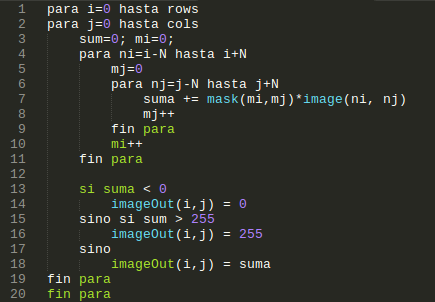
\includegraphics[scale=0.50]{./images/algoritmo.png}
	\caption{Pseudoc\'odigo que indica el procesdimiento para realizar la convoluci\'on entre la imagen y la m\'ascara, y la etapa de acotamiento.}
\end{figure}

Se aplicaron distintos operadores, cada uno con sus respectivas m\'ascaras.\\\\
\textbf{Operador de Roberts\\\\}
Las m\'ascaras para este operador se muestran en la Figura 4.

\begin{figure}[h]
	\centering
	\setlength{\unitlength}{0.00105in}
	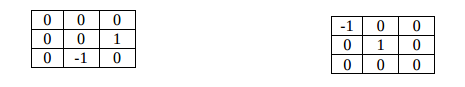
\includegraphics[scale=0.56]{./images/roberts.png}
	\caption{Gradiente fila y gradiente columna respectivamente.}
\end{figure}

Con estos gradientes se obtiene una buena respuesta a los bordes diagonales, esto debido a la disposici\'on de sus elementos en las m\'ascaras. Ofrece buenas prestaciones en cuanto a localizaci\'on.\\\\

\textbf{Operadores de Prewitt, Sobel y Frei-Chen\\\\}
Los tres operadores pueden formularse de forma conjunta ya que tienen una diposici\'on de sus elementos igual. Se utilizan las m\'ascaras de convoluci\'on mostradas en la Figura 5.

\begin{figure}[h]
	\centering
	\setlength{\unitlength}{0.00105in}
	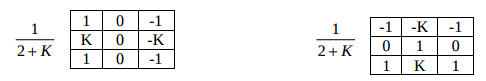
\includegraphics[scale=0.50]{./images/gradientes.png}
	\caption{Gradiente fila y gradiente columna respectivamente.}
\end{figure}

En el operador Prewitt ($k=1$) se involucran a los vecinos de filas/columnas adyacentes para proporcional mayor inmunidad al ruido.\\\\
El operador Sobel ($k=2$) en teor\'ia es m\'as sensible a los bordes diagonales que el operador de Prewitt pero en la pr\'actica hay poca diferencia entre ellos.\\\\
Frei-Chen ($k=\sqrt{2}$), el gradiente es el mismo para bordes verticales, horizontales y diagonales.\\\\

\section{Resultados}
Para realizar las pruebas se utilizar\'a s\'olo una imagen, esto debido a la cantidad de operadores.\\
La Figura 6. muestra la imagen que se utilizar\'a para las pruebas.\\

\begin{figure}[h]
	\centering
	\setlength{\unitlength}{0.00105in}
	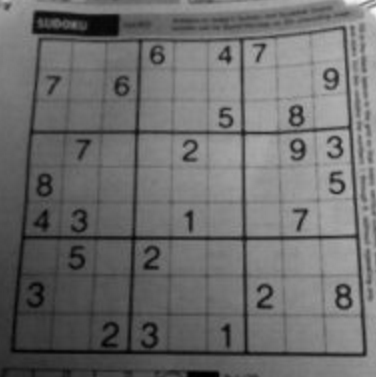
\includegraphics[scale=0.40]{./images/sudoku.png}
	\caption{Imagen de un juego de SuDoKu con caracter\'isticas interesantes para obtener mediante esta t\'ecnica.}
\end{figure}

\newpage
Al aplicar el gradiente de Prewitt los bordes se obtienen al realizar al convoluci\'on y obtener el gradiente utilizando las m\'ascaras vertical y horizontal.\\ Si se aplica el gradiente de Prewitt con la m\'ascara a $45$ grados se obtiene un resultado muy similar, ya que esta m\'ascara es una generalizaci\'on de las m\'ascaras vertical y horizontal. Esto se puede apreciar mejor en la Figura 7.

\begin{figure}[h]
	\centering
	\setlength{\unitlength}{0.00105in}
	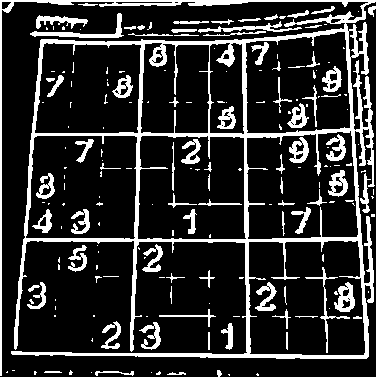
\includegraphics[scale=0.43]{./images/prewittXY.png}
	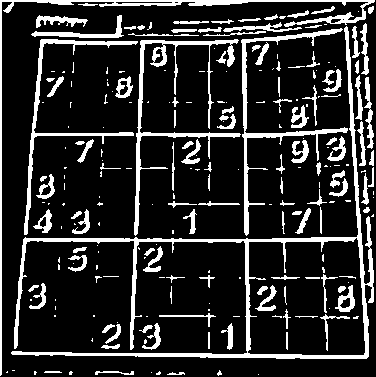
\includegraphics[scale=0.43]{./images/prewitt45.png}
	\caption{Bordes obtenidos con el gradiente de Prewitt horizontal y vertical, y a 45 grados respectivamente. }
\end{figure}

Si aplicamos el gradiente de Sobel y, de acuerdo a sus caracter\'isticas deber\'ia mostrar resultados semejantes al gradiente de Prewitt, aunque reduciendo el ruido ya que concentra los datos en el centro de la m\'ascara.

\begin{figure}[h]
	\centering
	\setlength{\unitlength}{0.00105in}
	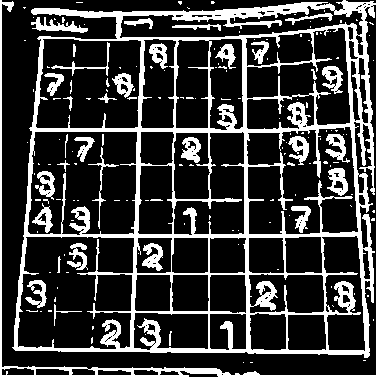
\includegraphics[scale=0.43]{./images/sobelXY.png}
	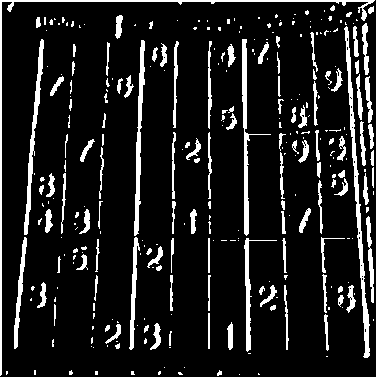
\includegraphics[scale=0.43]{./images/sobel45.png}
	\caption{Bordes obtenidos con el gradiente de Sobel horizontal y vertical, y a 45 grados respectivamente. }
\end{figure}

De acuerdo a la Figura 8. el resultado de aplicar la m\'ascara a 45 grados es muy distinta, ya que parece responder s\'olo a las lineales verticales y las horizontales las atenua. En cambio aplicando las m\'ascaras en horizontal y vertical se obtienen mejores resultados que utilizando el gradiente de Prewitt.
\newpage
\begin{figure}[h]
	\centering
	\setlength{\unitlength}{0.00105in}
	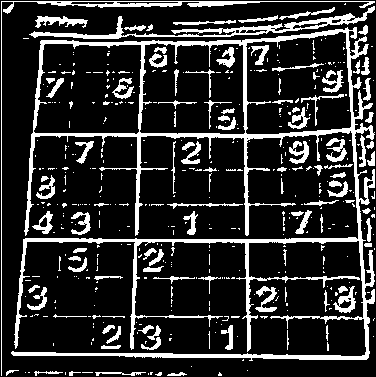
\includegraphics[scale=0.43]{./images/robertsXY.png}
	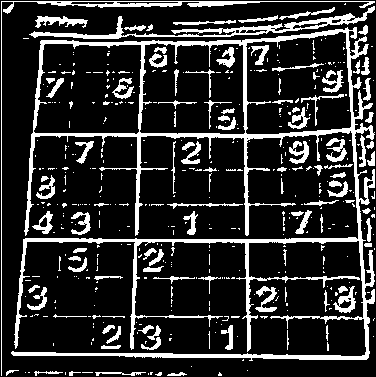
\includegraphics[scale=0.43]{./images/roberts45.png}
	\caption{Bordes obtenidos con el gradiente de Roberts horizontal y vertical, y a 45 grados respectivamente. }
\end{figure}

En la Figura 9. se muestra los resultados de aplicar el gradiente de Roberts. Los resultados son a\'un mejor que con el gradiente de Sobel. Se obtienen una mejora considerable al detectar la cuadricula del SuDoKu.\\\\

En la Figura 10. se muestra la imagen resultante de aplicar el gradiente de Frin-Chen.\\

\begin{figure}[h]
	\centering
	\setlength{\unitlength}{0.00105in}
	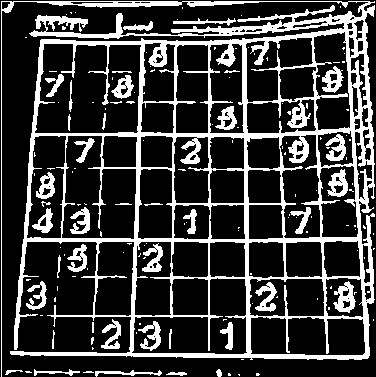
\includegraphics[scale=0.60]{./images/frinchenXY.png}
	\caption{Bordes obtenidos con el gradiente de Frin-Chen horizontal y vertical. }
\end{figure}

El gradiente de Frin-Chen es el gradiente que generaliza todos los dem\'as, y se puede observar en el resultado, es el gradiente que mejor detecta la cuadricula del SuDoKu y suprime el ruido mejor que los otros gradientes.\\\\

Los resultados de la Figura 7. y Figura 8. se obtuvieron umbralizando la imagen resultantes al obtener la magnitud del gradiente, el umbral utilizado fue 30. En cambio en la Figura 9. se utiliz\'o un umbral de 5.  Por \'ultimo, para la imagen resultado de la Figura 10. se utiliz\'o un umbral de 20.

\newpage
\section{Conclusiones}
En esta pr\'actica solo se mostraron cuatro tipos de gradientes para obtener los bordes de una imagen, en realidad son 8 filtros para cada gradiente, uno para cada 45 grados. Todos los gradientes se pueden utilizar para diferentes tipos de im\'agenes ya que se puede obtener resultados distintos dependiendo de la imagen y la m\'ascara utilizada.\\\\
Como resultado se obtienen diferentes bordes, aunque las diferencias son m\'inimas, en algunos casos se elimina el ruido de la imagen del resultado, como es el caso cuando se utiliza la m\'ascara de Sobel.\\\\
Otro dato importante es que al momento de umbralizar el valor del umbral afecta mucho al resultado de la imagen.

%$\begin{bmatrix}
% 1 & 1 & 1 & 1 \\
% 1 & 1 & 1 & 1 \\
% 1 & 1 & 1 & 1 \\
% 1 & 1 & 1 & 1 \\
%\end{bmatrix}$

%\begin{thebibliography}{1}
%    \bibitem{IEEEhowto:kopka}
%    H.~Kopka and P.~W. Daly, \emph{A Guide to \LaTeX}, 3rd~ed.\hskip 1em plus
%      0.5em minus 0.4em\relax Harlow, England: Addison-Wesley, 1999.
%\end{thebibliography}

%\begin{IEEEbiography}[{\includegraphics[width=1in,height=1.25in,clip,keepaspe%ctratio]{picture}}]{John Doe}
%\blindtext
%\end{IEEEbiography}

\end{document}